
\label{ch:rl}

In this chapter, we will introduce the theoretical bases of reinforcement learning, up to the Q-learning algorithm. This chapter serves as a starting point for the next one, which will regard the extension of the solution proposed here to tackle real world problems.
\section{Markov Decision Processes (MDP)}
\label{sec:MDP}
Before exploring the concept of Markov property and its implications, which are of paramount importance in the reinforcement learning problem, we will first analyze how the agent interacts with its surrounding environment.
\subsection{The Agent-Environment Interface}

The agent-environment interface is a way of better visualizing the RL problem, as in Figure \ref{fig:agentenvironment}\footnote{Source: \href{https://skymind.ai/wiki/deep-reinforcement-learning}{skymind.ai}}.

\begin{figure}[h!]
	\centering
	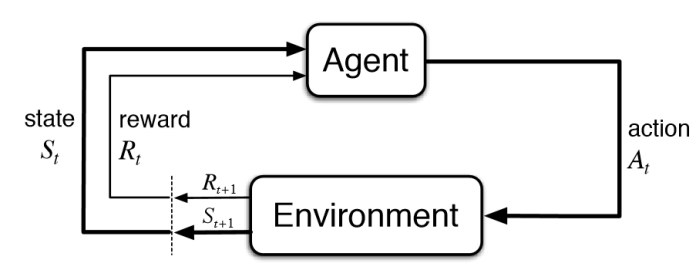
\includegraphics[width=12cm]{images/AgentEnvironment.jpg}
	\caption{The Agent-Environment interface}
	\label{fig:agentenvironment}
\end{figure}
 
The \textit{agent} is the entity acting on the \textit{environment}, that given a $state \ S_t \in \mathcal{S}$ selects one or more $actions \ A_t \in \mathcal{A}$ for interacting with the environment. Our agent then gets feedback from the environment itself: it gets a scalar valued $reward \ R_{t+1} \in \mathcal{R}$, and gets in a new state $S_{t+1} \in \mathcal{S}$. In a \textit{finite} MDP the set of states, actions and rewards ($\mathcal{S},\mathcal{A},\mathcal{R})$ contains a finite number of elements; nonetheless, the problem can be extended in the continuous case. The agent-environment feedback loop repeats over time and it is updated at each time \textit{step}: action selection, state and reward signals are sent only at specific moments in time (t = 0,1,2,3...). The sequence of actions, states and rewards defines a \textit{trajectory} in time that can be described as: 
\begin{equation}
	S_0, A_0, R_1, S_1, A_1, R_2, S_2, A_2, R_3... 
\end{equation}

\subsection{The Markov Property}
\label{sec:markov}
The Markov property is a fundamental concept in RL. The property states that a state $S_t$ is \textit{Markovian} if and only if:
\begin{equation}
	\mathbb{P}[S_{t+1} \,|\, S_t]  = \mathbb{P}[S_{t+1\,} |\, S_1, ..., S_t] 
\end{equation}
The meaning of this equation is that the probability of getting in a state $S_{t+1}$ given the current state $S_t$ is the same probability of getting in that state $S_{t+1}$ given the whole history of states $S_1, ..., S_t$. In other words, the meaning of a process following the Markov property is that future is independent of the past, given the present: hence, this allows us to ignore the history of all the preceding states, in order to decide what to do. Not only theoretically, but also practically speaking this makes the whole process of decision easier.


% MARKOVIANITY / NON EXAMPLES

\subsection{Returns and Rewarding Process}
Given one transition from state $S_t$ to state $S_{t+1}$, we have seen that a single reward is given to the agent. However, what we want to do in RL is to maximize the total sum of rewards $R$ over time. Therefore we define a total \textit{return} $G_t$ as:

\begin{equation}
	G_t  =  R_{t+1} + \gamma R_{t+2} + ...  =  \sum_{k=0}^{\infty}\gamma^k R_{t+k+1}
\end{equation}

Where $\gamma \in [0,1]$ is the \textit{discount factor}. This scalar value is very similar to the one used in economics: we are more interested in money returns which are close in time, but we are less interested in very long-term ones, because these could be just too late for us to benefit. This concept is well described by the sentence: "A dollar today is worth more than a dollar tomorrow". Moreover, discounting makes sense in a biological way since human and animal behavior tends to prefer immediate reward. We can extend this concept to reinforcement learning, by stating that our agent, i.e. Super Mario, will be more interested in getting a payoff as soon as possible, rather than waiting for thousands of time steps for a reward like a coin. Here is how value of $\gamma$ affects our evaluation:

\begin{itemize}
	\item $\gamma$ close to 0: our return evaluation will consider immediate rewards more important than future ones, thus leading to a "myopic" evaluation.
	\item $\gamma$ close to 1: the return function will take very  into account future rewards, thus leading to a "far-sighted" evaluation.
\end{itemize}

Myopic or far-sighted evaluations aside, the discounting process is very important in MDPs since we also avoid an infinite reward, impossible to handle practically speaking.

\subsection{Policies and Value Functions}
A \textit{policy} is the mapping from states to probabilities of selecting each possible action. If an agent at a time $t$ is following a policy $\pi$, then $\pi(a|s)$  describes the probability of taking action $a \in \mathcal{A}$ if it is in the state $s \in \mathcal{S}$:

\begin{equation}
	\pi(a|s)  =  \mathbb{P}[A_t  = a \, |\,  S_t=s]
\end{equation}
\\
\indent In MDPs, we can define the \textit{state-value function} $v_\pi(s)$ as the expected return starting from state $s$ and following policy $\pi$ thereafter:

%WRITE IN APPENDIX WHAT IS THE EXPECTATION


\begin{equation}
	v_\pi(s) \, = \, \mathbb{E}_\pi [G_t \, | \, S_t\,=\,s]
\end{equation}

We can also define an \textit{action-value function} $q_\pi(s,a$), the expected return starting from state $s$, taking action $a$, and then following policy $\pi$:

\begin{equation}
	q_\pi(s,a) = \mathbb{E}_\pi[G_t \, | \, S_t = s, A_t = a]
\end{equation}

\subsection{Bellman Equations}
The \textit{Bellman equations} define how to calculate the state-value functions and action-value functions in an iterative fashion. Since we can express $G_t = R_{t+1} + \gamma G_{t+1}$, then we can decompose the state-value function into immediate reward plus the discounted value of successor state:

\begin{equation}
	v_\pi(s) = \mathbb{E}_\pi[R_{t+1} + \gamma v_\pi (S_{t+1})\, | \, S_t = s]
\end{equation}

The action-value function can be similarly decomposed:

\begin{equation}
	q_\pi(s,a) = \mathbb{E}_\pi[R_{t+1} + \gamma v_\pi (S_{t+1},A_{t+1})\, | \, S_t = s, A_t = a]
\end{equation}

\subsection{Optimality Conditions}
The ultimate goal of RL is to obtain a policy which is \textit{optimal} in the sense that it is better in decision making than all other policies. We define the \textit{optimal state-value function} as:
\begin{equation}
	v_*(s) = \max_\pi v_\pi(s)
\end{equation}
In a similar way, the \textit{optimal action-value function} is defined as:
\begin{equation}
	q_*(s,a) = \max_\pi q_\pi (s,a)
\end{equation}
We define an ordering over policies: a policy is greater than another one if the values of all of its states are greater than those of the second one or that $\pi \geq \pi'$ if $v_\pi(s) \geq v_{\pi'}(s), \forall s$. For any Markov Decision Process:

\begin{itemize}
	\item An optimal policy $\pi_*$ such that it is better or equal to all other policies $\pi_* \geq \pi, \forall \pi$ exists
	\item All optimal policies achieve the optimal value function, $v_{\pi_*}(s)=v_*(s)$
	\item All optimal policies achieve the optimal action-value function, $q_{\pi_*}(s,a)=q_*(s,a)$.
\end{itemize}

Since the goal is finding the optimal policy, it can be found by maximizing over $q_*(s,a)$,

\begin{equation}
	\pi_*(a|s) = \begin{cases}
	1, & \text{if $a = \argmax_{a \in \mathcal{A}} \, q_*(s,a)$}\\
	0, & \text{otherwise}.
	\end{cases}
\end{equation}

This means that if the probability of the policy of selecting the best possible action is 1 . In order to find a solution for the Bellman Optimality Equation, which is not linear, many iterative solution methods have been developed. 

\subsection{Exploration and Exploitation}
\label{sec:explorationExploitation}
One of the most important problems in Reinforcement Learning, which does not have a single best answer, is the exploration and exploitation one. So far, we stated that the best way of choosing actions is to always select the action which seems optimal because it results in the highest reward: this is the \textit{exploitation} since the agent exploits what it thinks is the optimal solution.
\\
\indent However, during the learning process, it may be extremely important for the agent to sometimes choose the sub-optimal action because this may prevent it to get stuck in some local optimum. This is the process of \textit{exploration}. For example, if Super Mario has to reach the end flag of a level, maybe he knows the optimal path to get there in the least time possible. However, if he always did so, then he would never discover other possible better solutions like going down a pipe and earning a Star Coin first, or maybe just jumping onto a block and getting a tasty power-up. 
\\
\indent A widely used solution, called the \textit{$\varepsilon$-greedy} action selection, is not to always take the seemingly best action, but to take it with probability $1 - \varepsilon$, and to take a random action with probability $\varepsilon$:

\begin{equation}
\pi(a|s) = \begin{cases}
1 - \varepsilon, & \text{if $a = \argmax_{a \in \mathcal{A}} \, q_*(s,a)$}\\
\varepsilon, & \text{a random action}.
\end{cases}
\end{equation}

\section{Dynamic Programming}
One of the most important contributions to the RL research field is the Dynamic Programming (DP)\cite{bertsekas1995dynamic} approach. DP is a method for solving complex problems, by breaking them down into sub-problems, solving their sub-problems, and finally combining solutions to the sub-problems to solve the overall complex problem. Dynamic programming is a very general method for problems which have two main properties:

\begin{itemize}
		\item \textit{Optimal substructure}: if an optimal solution of the problem can be constructed from optimal solutions of its sub-problems. For example, if a car has to find the shortest path to a certain destination, then what can be done is to first find the shortest path a midpoint in the route, and then find the shortest path from the midpoint to the final destination.
		\item \textit{Overlapping problems}: the sub-problems which occur once, will occur again and again. In the car example, we broke down the problem into two sub-problems: getting from the starting point to a midpoint, and from the midpoint to the end. This solution will help to solve the sub-problem of how to get from another point to the final destination: solutions can thus be cached and reused.
\end{itemize}

As it turns out, Markov Decision Processes satisfy both the aforementioned properties. The Bellman Equation results in a recursive decomposition: it breaks down the calculation in two parts, the optimal behavior for one step followed by the optimal behavior after that step. The overlapping problems solution in MDPs is given by the value function: it is like a cache of the information we have collected about the MDP. In the car example, after figuring out the optimal path to the final destination, that information is store: when we need that datum for a similar path, we will have already computed it and we will not need to recompute it.

\subsection{Dynamic Programming Shortcomings}
Although it introduces useful tools for solving reinforcement learning problems, DP has important shortcomings. Firstly, DP methods are \textit{model based} and require a complete knowledge of the environment, such as transition probabilities and rewards. Secondly, they suffer from the \textit{curse of dimensionality} since, having to perform a complete backup of all states and transition, increasing the state and action spaces dimensions will exponentially increase the calculations required for solving the problem; which becomes impossible if the dimensionality approaches infinity in continuous spaces.

\subsection{Generalized Policy Iteration}
\label{sec:gpi}
Before going to explore the Monte Carlo methods and following algorithms that try to solve the curse of dimensionality, we need to introduce the Generalized Policy Iteration (GPI), which is an iterative scheme composed of two steps:
\begin{itemize}
	\item \textit{Policy evaluation step}: an approximation of the value function based on the current policy is created .
	\item \textit{Policy improvement step}: the policy is improved with respect to the current value function, by acting greedily on it.
\end{itemize}

This process will always converge, after a number of iterations, to the optimal policy $\pi_*$.


\section{Monte Carlo Methods}
The idea behind Monte Carlo (MC)\cite{metropolis1949monte} methods was derived from the same-name casino: finding out a way of solving a problem by using a major random component. Monte Carlo methods work on the concept of GPI of Section \ref{sec:gpi}: they learn value functions from direct interaction with the environment by means of episodes of experience; performing random rollouts on the system and by updating the accumulation of rewards and the distribution of states encountered at the end of the episode. The current policy is then estimated by making it directly greedy with respect to the current value function. Using these two steps iteratively, it can be shown that the algorithm converges to the optimal value function and policy.
\\
\indent Since they do not require a model, Monte Carlo methods are \textit{model-free} ones, thus they have a major advantage with respect to the model-based Dynamic Programming. A simple every-visit MC method calculating the value of a state is:

\begin{equation}
	V(S_t) \gets V(S_t) + \alpha[G_t - V(S_t)]
	\label{eq:MC}
\end{equation}

where $G_t$ is the actual return at time $t$, and $\alpha \in (0,1]$ is the \textit{learning rate}, a step-size parameter indicating how much we shift our estimate $V(S_t)$ towards a more realistic value based on the calculation of the actual return. As it can be noticed, the value of $G_t$ can only be computed at the end of the episode, so value updates will happen only at that moment.
\\
\indent Although MC methods are relatively simple and straightforward in their implementation, they require a large number of iterations for their convergence and suffer from a large variance in their value function estimation: hence, they cannot be considered efficient for the majority of RL purposes. Nonetheless, they are conceptually very important in the development of more complex algorithms.

\section{Temporal Difference Methods}

Temporal Difference (TD) methods combine concepts from both Dynamic Programming and Monte Carlo methods in order to avoid some of the shortcomings of both methods. TD builds on the same idea of Generalized Policy Iteration, but differs from Monte Carlo in the policy evaluation step. Whereas MC methods use the total accumulated reward $G_t$ to make predictions and have to wait until the end of the episode, as seen in Equation \ref{eq:MC}, TD methods only need to wait until the next time step for updating. The simplest TD method makes the update:

\begin{equation}
V(S_t) \gets V(S_t) + \alpha[R_{t+1} + \gamma V(S_{t+1}) - V(S_t)]
\label{eq:TD}
\end{equation}

immediately on transition $S_{t+1}$ and receiving $R_{t+1}$, and does not have to wait until the end of the episode knowing a better estimate of our state value. The quantity in the brackets can be seen as a sort of error since it is the difference between $R_{t+1} + V(S_{t+1})$, the new estimate, and $V(S_t)$, the old estimate. This quantity called \textit{TD error} is important in many reinforcement learning algorithms:

\begin{equation}
	\delta _t \doteq R_{t+1} + \gamma V(S_{t+1}) - V(S_t)
\end{equation}
\\
\indent Like in Monte Carlo methods, TD learns directly from episodes of experience, and being \textit{model-free}, it has a major advantage in environments where MDP transitions and rewards are not known. However, Temporal Difference methods have a major advantage over MC ones: they can learn by \textit{incomplete} sequences of episodes, by \textit{bootstrapping}. Bootstrapping is the idea of updating a guess, $V(S_t)$, towards a guess,  $R_{t+1} + \gamma V(S_{t+1})$: this way, we do not have to wait until the end of an episode.
\\
\indent For example, suppose you want to drive home and the navigation algorithm tells you will take 30 minutes to get there. But then, after 5 minutes, you are stuck in a traffic jam, which will add another 30 minutes to your commuting. A Monte Carlo algorithm would have to wait until you have reached home, finishing your "episode", to update its estimate. In contrast, a TD one would update the estimated time to arrival in real time, telling that you will have another 55 minutes driving home. As a result, the latter method is much more useful in this real life application.
\\
\indent Two TD algorithms which have been widely used to solve RL problems are \textit{SARSA} and \textit{Q-Learning} will be explored in the next chapters.

\subsection{SARSA}

SARSA (\textit{State-Action-Reward-State-Action}) is an on-policy temporal difference algorithm which tries to learn an action value function, instead of the value one. The policy evaluation step uses the TD error for the action value function, which is similar to the value function. SARSA is an \textit{on-policy} learner since it learns the value function of the current policy; in contrast, an \textit{off-policy} learner learns the value functions of the optimal policy while following another one.
\\
\indent The idea behind SARSA is choosing actions with an \textit{$\varepsilon$-greedy} policy and then updating the value of the action value function $Q(s_t, a_t)$, which is the value of being in state $s$ at time $t$ and taking action $a$, after observing the reward $r_{t}$ and the state we reach at time $t+1$,  $s_{t+1}$. The algorithm is summarized below in pseudo code:

\begin{algorithm}
	\caption{SARSA}
	\SetAlgoLined
	\DontPrintSemicolon
	Initialize $Q(s,a)$ randomly\;
	\Repeat{terminated}{
	Observe initial state $s_1$\;
	\For{t=1: T}{
	Select an action $a_1$ using policy derived from Q (e.g. $\varepsilon$-greedy)\;
	Carry out action $a_t$\;
	Observe reward $r_t$ and new state $s_{t+1}$ \;
	Update Q using 
	% MATCH SYNTAXXX!! LIKE s'
	\begin{equation} 
		Q(s_t, a_t) \gets Q(s_t,a_t) + \alpha[r +  \gamma Q(s_{t+1}, a_{t+1}) - Q(s_t,a_t)]		
	\end{equation}
}
}
\end{algorithm}



\subsection{Q-Learning}
\label{sec:qlearning}

Q-Learning\cite{watkins1992q} is one of the simplest but still quite efficient algorithms, and one of the earliest breakthroughs in Reinforcement Learning. It is an off-policy TD control algorithm which is similar to SARSA but differs in the way the action value funtion $Q(s_t, a_t)$ is updated (see Algorithm \ref{alg:Qlearning}.)

\begin{algorithm}[H]
	\label{alg:Qlearning}
	\caption{Q-learning}
	\SetAlgoLined
	\DontPrintSemicolon
	Initialize $Q(s,a)$ randomly\;
	\Repeat{terminated}{
		Observe initial state $s_1$\;
		\For{t=1: T}{
			Select an action $a_1$ using policy derived from Q (e.g. $\varepsilon$-greedy)\;
			Carry out action $a_t$\;
			Observe reward $r_t$ and new state $s_{t+1}$\;
			Update Q using 
			% MATCH SYNTAXXX!! LIKE s'
			\begin{equation} 
			Q(s_t, a_t) \gets Q(s_t,a_t) + \alpha[r + \max_a \gamma Q(s', a) - Q(s_t,a_t)]	
			\label{eq:Qlearning}	
			\end{equation}
		}
	}
\end{algorithm}

As we can notice in Equation \ref{eq:Qlearning}, the most important difference between SARSA and Q-Learning is the update rule; while in the former the action value function is updated based on the current policy, Q-Learning updates $Q(s_t, a_t)$ directly greedily follow another policy that is, for example, an $\varepsilon$-greedy one.
\\
\indent These algorithms have proven very efficient in low dimensional state and action spaces. However, for real life applications, the number of states and/or actions greatly exceeds what we can consider of low dimensionality. Therefore, we will need further tweaking methods for an actual implementation of these algorithms.

